% LoVullo Specification Specification
%
% Yep.

\documentclass[draft]{lvspec}
\usepackage{multicol}
\usepackage[final]{graphicx}

\makeatletter
  \def\@lvspec@titlecmd{%
    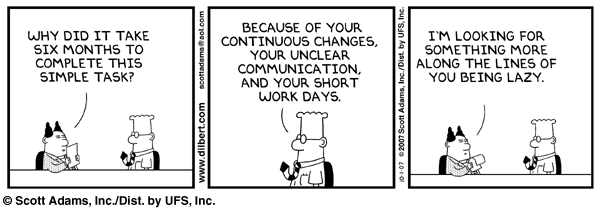
\includegraphics[scale=0.5]{images/dilbert-time.png}
    \vfill
  }%
\makeatother

\begin{document}

\title{LoVullo Specification Specifications}
\author{Mike Gerwitz}
\abstract{%
  \setlength\columnsep{-5ex}%
  \begin{multicols}{2}
  \begin{quote}
    \sl\small\raggedright
    \def\ind{}%
    %
    In the beginning was the plan,\\
    \ind and then the specification;\\
    And the plan was without form,\\
    \ind and the specification was void.

    And darkness\\
    \ind was on the faces of the implementors thereof;\\
    And they spake unto their leader, saying:\\
    ``It is a crock of shit,\\
    \ind and smells as of a sewer.''

    And the leader took pity on them,\\
    \ind and spoke to the project leader:\\
    ``It is a crock of excrement,\\
    \ind and none may abide the odor thereof.''

    And the project leader\\
    \ind spake unto his section head, saying:\\
    ``It is a container of excrement,\\
    \ind and it is very strong, such that none may abide it.''

    The section head then hurried to his department manager,\\
    \ind and informed him thus:\\
    ``It is a vessel of fertilizer,\\
    \ind and none may abide its strength.''
    \goodbreak

    The department manager carried these words\\
    \ind to his general manager,\\
    and spoke unto him\\
    \ind saying:\\
    ``It containeth that which aideth the growth of plants,\\
    \ind and it is very strong.''

    And so it was that the general manager rejoiced\\
    \ind and delivered the good news unto the Vice President.\\
    ``It promoteth growth,\\
    \ind and it is very powerful.''

    The Vice President rushed to the President's side,\\
    \ind and joyously exclaimed:\\
    ``This powerful new software product\\
    \ind will promote the growth of the company!''

    And the President looked upon the product,\\
   \ind and saw that it was very good.

   \hfill---The Jargon File
  \end{quote}
  \end{multicols}
  \bigskip
}
\maketitle

\end{document}
